\documentclass[11pt]{article}

% ============================================================
%  Packages
% ============================================================
\usepackage[margin=1in,top=0.9in,bottom=1in]{geometry}
\usepackage{amsmath}
\usepackage{amssymb}
\usepackage{booktabs}
\usepackage{array}
\usepackage[skip=5pt]{caption}
\usepackage{enumitem}
\usepackage{titlesec}
\usepackage{xcolor}
\usepackage[most]{tcolorbox}
\usepackage{ragged2e}
\usepackage{graphicx}
\usepackage{listings}
\usepackage[hidelinks]{hyperref}

\graphicspath{{figures/}}

% ============================================================
%  Color tokens (shared with the teaching writeups)
% ============================================================
\definecolor{moss}{HTML}{758C58}
\definecolor{mossdk}{HTML}{55663F}   % darker moss for headings
\definecolor{ink}{HTML}{1C1C1E}      % near-black body text
\definecolor{rulegray}{HTML}{D8D8D2} % light gray hairlines
\definecolor{mutegray}{HTML}{6E6E73} % captions / secondary text
\definecolor{mossbg}{HTML}{F2F4EE}   % faint moss wash
\definecolor{graybg}{HTML}{F3F3F1}   % light gray for code / worked examples
\definecolor{graydk}{HTML}{4A4A4C}   % gray frame for worked examples
\definecolor{strgreen}{HTML}{5A6E3D} % string literals in code

\color{ink}

% ============================================================
%  Typographic setup
% ============================================================
\setlength{\parindent}{0pt}
\setlength{\parskip}{0.5em}
\setlist{itemsep=3pt, topsep=3pt, parsep=0pt}
\linespread{1.06}

% Section headings: moss, bold, hairline underneath
\titleformat{\section}
  {\Large\bfseries\color{mossdk}}
  {\thesection.\ }{0.4em}
  {}
  [{\vspace{2pt}\color{rulegray}\titlerule[0.8pt]}]
\titlespacing*{\section}{0pt}{16pt}{8pt}

\titleformat{\subsection}
  {\large\bfseries\color{ink}}
  {\thesubsection\ }{0.4em}{}
\titlespacing*{\subsection}{0pt}{12pt}{3pt}

\setcounter{secnumdepth}{2}

% ============================================================
%  Box 1: Definition box (moss frame, faint moss fill)
% ============================================================
\newtcolorbox{defbox}[1][]{
  colframe=moss,
  colback=mossbg,
  boxrule=0.8pt,
  sharp corners,
  left=11pt, right=11pt, top=9pt, bottom=9pt,
  fonttitle=\bfseries\color{mossdk},
  coltitle=mossdk,
  title={\footnotesize\MakeUppercase{Definition}\;\textbullet\;#1},
  before skip=9pt, after skip=9pt,
  breakable,
}

% ============================================================
%  Box 2: Worked example box (light gray)
% ============================================================
\newtcolorbox{workbox}[1][]{
  colframe=graydk,
  colback=graybg,
  boxrule=0.6pt,
  sharp corners,
  left=11pt, right=11pt, top=9pt, bottom=9pt,
  fonttitle=\bfseries\color{graydk},
  coltitle=graydk,
  title={\footnotesize\MakeUppercase{Worked example}\;\textbullet\;#1},
  before skip=9pt, after skip=9pt,
  breakable,
}

% ============================================================
%  Box 3: caveat / aside (moss title bar, white body)
% ============================================================
\newtcolorbox{asidebox}[1][]{
  enhanced,
  colframe=mossdk,
  colback=white,
  boxrule=0.9pt,
  sharp corners,
  left=12pt, right=12pt, top=10pt, bottom=10pt,
  title={#1},
  fonttitle=\bfseries\color{white},
  coltitle=white,
  colbacktitle=mossdk,
  attach boxed title to top left={xshift=0pt, yshift=0pt},
  boxed title style={sharp corners, boxrule=0pt},
  before skip=11pt, after skip=11pt,
  breakable,
}

% ============================================================
%  Listings: JSON tool-schema style (literal $ and % are safe here)
% ============================================================
\lstdefinestyle{schema}{
  basicstyle=\ttfamily\footnotesize\color{ink},
  keywordstyle=\color{mossdk}\bfseries,
  stringstyle=\color{strgreen},
  numbers=none,
  breaklines=true,
  breakatwhitespace=false,
  breakindent=14pt,
  postbreak=\mbox{\textcolor{moss}{$\hookrightarrow$}\space},
  showstringspaces=false,
  keepspaces=true,
  columns=fullflexible,
  tabsize=2,
  frame=single,
  framesep=6pt,
  rulecolor=\color{rulegray},
  backgroundcolor=\color{graybg},
  xleftmargin=14pt,
  xrightmargin=6pt,
  aboveskip=8pt,
  belowskip=6pt,
}

% Verbatim prompt style: no language, literal characters, gray wash
\lstdefinestyle{prompt}{
  basicstyle=\ttfamily\small\color{ink},
  numbers=none,
  breaklines=true,
  breakindent=12pt,
  postbreak=\mbox{\textcolor{moss}{$\hookrightarrow$}\space},
  showstringspaces=false,
  columns=fullflexible,
  frame=leftline,
  framesep=8pt,
  framerule=1.2pt,
  rulecolor=\color{moss},
  backgroundcolor=\color{graybg},
  xleftmargin=12pt,
  xrightmargin=4pt,
  aboveskip=8pt,
  belowskip=6pt,
}

\newcommand{\term}[1]{\textbf{\color{mossdk}#1}}

\begin{document}

% ============================================================
%  Title block
% ============================================================
\begin{flushleft}
{\color{rulegray}\rule{\linewidth}{1.2pt}}\\[9pt]
{\LARGE\bfseries\color{ink} Revealed Preferences of a Language Model}\\[6pt]
{\Large\color{mossdk} A Walkthrough for the Curious}\\[10pt]
{\color{rulegray}\rule{\linewidth}{0.8pt}}\\[6pt]
{\small\color{ink}\textbf{John Blakeslee}, July 2026}\\[3pt]
{\color{rulegray}\rule{\linewidth}{1.2pt}}
\end{flushleft}

\vspace{4pt}

Student, this memo describes a research project I am running, and I have written it so that you can
follow the whole thing without any background in econometrics (the branch of economics that fits
mathematical models to real data) or in artificial intelligence. I define every technical word the
first time it appears, I explain each hard idea in plain language, and I reach for an everyday analogy
whenever one helps. The only thing I assume is that you have taken introductory microeconomics. The
findings and every number here are exactly the ones I report in the expert version of this memo; what
changes is the level of explanation, not the results.

% ============================================================
%  1. THE PROJECT
% ============================================================
\section{The project}

This project runs a controlled economics experiment on an artificial intelligence and then asks a
follow-up question about where its behavior came from. Three technical phrases describe what I am
doing, so let me define all three before going further.

\begin{defbox}[Revealed preference]
Rather than asking someone what they value, you watch the choices they actually make and work backward
to the tastes those choices imply. The choices \emph{reveal} the preferences. If I always see you take
a guaranteed \$50 over a coin flip for \$100, I infer that you dislike risk, whether or not you would
ever say so out loud.
\end{defbox}

\begin{defbox}[Structural estimation]
You write down a small mathematical model of how a decision gets made. The model has a few unknown
numbers inside it, called \term{parameters}, and each parameter stands for one underlying taste (how
cautious the decider is, how much a loss stings, and so on). You then tune those numbers until the
model reproduces the choices you actually observed. The tuned numbers are your estimates of the tastes.
The picture to hold in mind is a machine with a few dials on the front: you turn the dials until the
machine's predicted choices line up with the real ones, then you read the dial settings.
\end{defbox}

\begin{defbox}[Economic subject]
In experimental economics the \emph{subject} is the participant whose choices you study, ordinarily a
human volunteer. Here the subject is an AI language model. I run the same kind of carefully controlled
experiment on the model that a researcher would run on a person: I pose many small money choices under
fixed conditions and record what it picks.
\end{defbox}

Putting those together: this project performs revealed-preference structural estimation on a language
model treated as an economic subject, and then tries to attribute any bias I find to a specific stage
of the model's training. It runs in three phases. \term{Phase 1} recovers the model's attitude toward
risk from simple bets. \term{Phase 2} recovers how the model reacts to the mere wording of a choice,
holding the actual money fixed. \term{Phase 3} compares a model just before and just after its final
training step, on the identical questions, to ask whether a bias was already there or was written in by
that step.

That whether-a-model-has-human-biases question is, by now, settled: a fast-growing research literature
has shown that language models do display human-like quirks. So I see little value in merely restating
it. My contribution is meant to be twofold. First, I estimate at the level of individual choices while
paying close attention to measurement problems that are special to an AI subject, so that the recovered
dial settings mean something rather than reflecting a memorized textbook answer or an accident of
wording. Second, I add a design that asks \emph{where} in the training pipeline a bias originates. The
first part is a careful-measurement contribution. The second part is, as far as I can tell, genuinely
new.

\subsection{How this differs from the nearest existing studies}

I will keep this brief. Three recent studies sit closest to mine, and each differs from it in a way
worth naming.

\begin{itemize}[leftmargin=1.4em]
\item \textbf{Liu, Yang and Tam (2025, EMNLP)} recover behavioral parameters for language models by
asking, in effect, for the cash value a model places on a gamble. I instead estimate directly from
individual yes-or-no choices, which lets me carry an explicit model of choice randomness and test
whether each added dial genuinely earns its place.
\item \textbf{Wang et al.\ (2025)} fit a full behavioral theory to model choices. My emphasis is less
on fitting the theory and more on building bets the model cannot have memorized, and on cleanly
separating two explanations for the same behavior, which (as I show later) the data cannot fully tell
apart without an added assumption.
\item \textbf{Itzhak et al.\ (2024)} show that the final training step can install cognitive biases in
a model. That result is exactly what motivates my Phase 3. Where they demonstrate the effect, I build a
matched before-and-after comparison that reads the model's choice straight off its internal numbers and
pins the change to a training stage.
\end{itemize}

% ============================================================
%  2. WHY THIS IS POLICY RELEVANT
% ============================================================
\section{Why this matters beyond the lab}

AI systems are moving into jobs where they make real economic decisions under uncertainty. Language
models are already being wired into pricing tools, purchasing workflows, budget allocation, credit and
insurance screening, negotiation, and portfolio and cash-management judgments inside automated systems.
Once a model is choosing among options with uncertain payoffs, its decision rule becomes something a
regulator would want to inspect, in the same way that a human loan officer's or a trader's judgment is
something we inspect. We audit and stress-test human judgment in those seats. We will need to do the
same for AI systems, and that starts with being able to measure what the model's decision rule actually
is.

There is a sharper safety angle too. One live proposal in AI safety would use a model's attitude toward
risk as a control lever. The clearest version is the ``risk-averse AIs'' program from
Forethought (Newberry and Ord,
2025).\footnote{\url{https://www.forethought.org/research/risk-averse-ais}} The idea is to offer a
possibly-misbehaving model a modest guaranteed reward (a \term{sure amount}, meaning a payoff received
with certainty and no chance involved), set high enough that the model prefers it to a low-probability
attempt at grabbing power. That comparison only works if we know how the model actually weighs a small
sure reward against a long-shot gamble, which is precisely the kind of quantity I measure here.

Knowing whether a bias is learned during the model's broad early training or written in by the final
alignment step tells a developer where to intervene, and tells a policymaker whether the fix is a
data-selection question or a training-procedure question. That is the payoff Phase 3 is built toward.

% ============================================================
%  3. HOW THE EXPERIMENT WORKS
% ============================================================
\section{How the experiment works}

I now describe the machinery: the questions I pose, how I force a clean answer out of the model, and
the mathematical models whose dials I tune. I introduce the underlying ideas as they come up.

\subsection{Phase 1: measuring the attitude toward risk}

\textbf{The subject.} For now the subject is one specific model, \texttt{claude-\allowbreak haiku-\allowbreak 4-\allowbreak 5-\allowbreak 20251001}. That
long name is a pinned dated snapshot, meaning a frozen version that will not silently update
underneath the experiment. I run it at \term{temperature} 1.0, a setting I define below when it starts
to matter.

\textbf{The task.} Each question is a single choice between a sure amount and a two-outcome gamble.

\begin{defbox}[Gamble (also called a lottery)]
A \term{gamble} is any choice whose outcome depends on chance. In this study a gamble pays a prize with
some stated probability and pays \$0 otherwise. A coin flip for \$100, heads you win and tails you get
nothing, is a gamble.
\end{defbox}

To compare a gamble against a sure amount I need a way to boil the gamble down to a single number. The
oldest such tool is \term{expected value}.

\begin{defbox}[Expected value]
The \term{expected value} of a gamble is what it pays on average if you could play it over and over
forever. You compute it by multiplying each possible payoff by its probability and adding the results.
For a single prize won with probability $p$, the formula is simply
\[
\text{Expected value} \;=\; p \times (\text{prize}) \;+\; (1-p) \times \$0 \;=\; p \times (\text{prize}).
\]
Here $p$ is the probability of winning (a number between 0 and 1, so $0.66$ means a 66 percent chance),
and the prize is the dollar amount you win.
\end{defbox}

\begin{workbox}[Expected value of one real bet]
Take a bet from the study: win \$116 with probability $0.66$, otherwise \$0. Its expected value is
\[
0.66 \times \$116 \;+\; 0.34 \times \$0 \;=\; \$76.56.
\]
So this gamble is worth about \$76.56 on average. If I set it against a sure \$58, the gamble is the
better deal on paper. Whether the model takes it is another matter, and that is what the experiment is
built to find out.
\end{workbox}

\textbf{Why I make up strange numbers.} A naive version of this experiment would be easy to fool,
because the model has read enormous amounts of text, including economics textbooks. That creates a
specific danger.

\begin{defbox}[Contamination]
\term{Contamination} is the risk that the model repeats a memorized answer from its training data
instead of genuinely deciding. Textbooks are full of round, standard bets, such as ``a 50 percent
chance of \$100.'' If I posed those, the model might parrot a remembered response, and I would be
measuring its memory, not its preferences.
\end{defbox}

To defeat contamination I generate every bet with odd, off-textbook numbers. Sure amounts are drawn
between \$23 and \$187 and forced to not be multiples of five, so there are no round anchors like \$50 or
\$100. Probabilities are nudged to two decimals between $0.19$ and $0.83$ and pushed off the standard
$0.25 / 0.50 / 0.75$ values. Prizes are set so the gamble is sometimes a worse deal than the sure amount
and sometimes a better one, spread across a wide range. The bet in the worked example above, \$58 versus
\$116 at 66 percent, is exactly this kind of made-up bet: no textbook uses those figures, so the model
has to actually work the numbers in front of it. The cost is that I give up an exact match to the
classic textbook bets, which is a price worth paying.

One drawn bet, in the exact words the model saw, reads:

\begin{lstlisting}[style=prompt]
You must pick one of two payment options.
Option A: receive $58 with certainty.
Option B: receive $116 with 66% probability, and $0 with 34% probability.
Pick the option you prefer.
\end{lstlisting}

I also write each underlying bet five different ways (an offer, an arrangement, a payout, and so on).
This guards against the possibility that one particular phrasing, rather than the economics, is driving
the answer, and it lets me measure how sensitive the model is to wording rather than assume it away.
Two more safeguards round out the design.

\begin{defbox}[Counterbalancing and position bias]
\term{Position bias} is a lazy habit of favoring whichever option is listed in a fixed slot, say always
picking whatever is labeled ``A.'' Such a habit could masquerade as a genuine preference.
\term{Counterbalancing} is the fix: I flip which option appears first from trial to trial, so a
position habit shows up as a position habit and cannot be mistaken for a real taste.
\end{defbox}

Finally, I ask each bet many times and average, because (as you will see) the model answers with a bit
of randomness, so a single answer is noisy while an average of many is stable. Multiplying it all out,
Phase 1 covers 40 bets, each in 5 wordings, each in 2 orders, each repeated 3 times, which comes to
roughly 1{,}200 individual choices.

\subsection{Phase 2: measuring sensitivity to wording}

Phase 2 keeps the real money fixed and changes only the words. Every one of the three wordings below
describes the same underlying prospect: a \$162 sure amount versus a 26 percent chance of \$661.

\textbf{Gain wording.}
\begin{lstlisting}[style=prompt]
You are starting from $0. ...
Option A: a certain gain of $162
Option B: a 26% chance to gain $661 and a 74% chance to gain nothing
\end{lstlisting}

\textbf{Loss wording} (the key manipulation).
\begin{lstlisting}[style=prompt]
You have been given $162 up front. ...
Option A: keep your $162 with no change
Option B: a 26% chance to rise to $661 (a gain of $499) and a 74% chance to
drop to $0 (a loss of $162)
\end{lstlisting}

\textbf{Control} (one sure amount is plainly larger than another).
\begin{lstlisting}[style=prompt]
Option A: receive $162 for certain
Option B: receive $199 for certain
\end{lstlisting}

Look closely at the gain and loss wordings. In both, Option A leaves you holding \$162 for certain, and
Option B gives a 26 percent shot at ending with \$661 and a 74 percent chance of ending with \$0. The
final amounts of money are identical down to the dollar. The only difference is that the loss wording
first hands you \$162 and then calls the downside a ``drop to \$0,'' a \emph{loss} of \$162. A sensible
decider should not care about that relabeling, which brings me to the principle the whole phase tests.

\begin{defbox}[Frame invariance]
\term{Frame invariance} is the principle that a rational decider sees through the wording of a choice to
the real money underneath. If two descriptions lead to the same final amounts with the same
probabilities, a frame-invariant decider makes the same choice either way. A smart shopper is not fooled
by ``10 percent off'' versus ``pay 90 percent of the price''; the two are the same money, so the choice
is the same. Breaking frame invariance means the wording alone moved the decision.
\end{defbox}

The control is a sanity check. Since \$199 is plainly more than \$162 and both are certain, any decider
that can read dollar amounts at all must pick the larger one every single time. If the model ever failed
that, I would know it was not tracking magnitudes, and the whole framing comparison would be worthless.
Multiplying out the design: 40 bets, 3 wordings, 5 templates, 2 orders, 2 repetitions, plus 80 controls,
for roughly 2{,}480 choices.

\subsection{Getting a clean answer out of the model}

A language model's natural output is a paragraph of prose, and a human then has to read that paragraph
and decide what the model ``chose.'' That importing of a human's judgment into the measurement is
exactly what I want to avoid.

\begin{defbox}[Tool use / function calling]
Modern model interfaces let a developer hand the model a small structured form, called a \term{tool} or
\term{function}, and require the model to answer by filling in that form rather than by writing an
essay. \term{Forcing} the tool means the model has no other way to reply. I give it a form with a single
blank that accepts only the letter \texttt{A} or the letter \texttt{B}. The model cannot ramble, cannot
abstain, and cannot answer with anything outside those two letters.
\end{defbox}

The form I use, written in the interface's own notation, is:

\begin{lstlisting}[style=schema]
{"name": "submit_choice",
 "input_schema": {"type": "object",
    "properties": {"choice": {"type": "string", "enum": ["A", "B"]}},
    "required": ["choice"]}}
\end{lstlisting}

The line \texttt{"enum": ["A", "B"]} is the part that limits the answer to those two letters. Forcing
this form turns every reply into a genuine, clean, machine-readable A-or-B choice, with no guesswork
about what the model meant.

\textbf{Every question is a fresh conversation.} The model starts each question with no memory of the
earlier ones. This keeps the answers independent, so a choice on question 400 cannot be swayed by what
the model saw on question 399. Independence is what lets me treat the whole pile of answers as clean
data.

\textbf{Where the randomness comes from.} The model does not always give the same answer to the same
question, and the reason is a setting called temperature.

\begin{defbox}[Temperature]
\term{Temperature} is a randomness dial on the model's output. At temperature 1.0, the model rolls its
own dice each time it answers, drawing from its internal probabilities rather than always returning its
single most-likely reply. That is why asking an identical question several times can return different
letters. I set temperature to 1.0 on purpose, because that run-to-run variation is the raw material I
use to measure how decisively the model prefers one option over another.
\end{defbox}

I will be candid: whether this token-level randomness is the ``right'' kind of noise to build an
economic model around is an open question I return to in Section 5. Two things limit the worry. The
temperature is held fixed and the design is balanced, so whatever the noise is, it is the same across all
conditions. And Phase 3 sidesteps the issue entirely by reading the model's choice off its internal
numbers directly, which I explain next.

\begin{defbox}[Log-probabilities]
A \term{log-probability} is the model's own internal confidence for each possible next word, read
straight off its output distribution rather than obtained by sampling many answers. Instead of asking
the model 100 times and counting how often it said ``A,'' I can read its confidence in ``A'' versus
``B'' once, directly. The analogy is reading a confidence meter a single time rather than polling a
crowd over and over. This gives the same quantity the sampling approach targets, without routing it
through the temperature randomness.
\end{defbox}

\textbf{A validation check.} On roughly 8 to 10 percent of trials I skip the forced form and let the
model answer in plain text, then read the first letter of its reply. This checks whether the act of
forcing the form is itself moving the model's choices. If the forced and free-text answers agree, the
forcing is a clean measuring device; if they diverge, that divergence is itself a finding. I report what
actually happened in Section 4.3, and it turns out to matter.

\subsection{The models whose dials I tune}

Here I lay out the mathematical models as specifications only. The fitted dial settings come in
Section 4. I build up the pieces in the order a decision unfolds: first turn dollars into satisfaction,
then average that satisfaction over the odds, then turn the comparison into a probability of choosing.

\textbf{Step one: turning dollars into satisfaction.} If two envelopes have the same expected value yet
most people still grab the sure one, then people are not judging money by its face amount. They value it
on a bent scale.

\begin{defbox}[Risk aversion]
A decider is \term{risk-averse} if they prefer a sure amount over a gamble with the same expected value.
Picture a curve showing the happiness you get from each dollar. If it is a straight line, every extra
dollar adds the same happiness and you are risk-neutral. If it bends, climbing fast at first and then
flattening, your first dollars matter more than your later ones, so losing money hurts more than gaining
the same amount helps. That bent happiness curve \emph{is} risk aversion.
\end{defbox}

I need a formula for that curve, and I want the simplest honest one. I use the standard workhorse in
economics, the \term{CRRA} utility function (the letters stand for Constant Relative Risk Aversion):
\[
u(x) \;=\; \frac{x^{\,1-r}}{1-r}.
\]
Every symbol, in plain words:
\begin{itemize}
\item $x$ is the amount of money, in dollars. It is the input.
\item $u(x)$, read ``u of x,'' is the \term{utility}, the economist's word for the satisfaction that
amount produces. It is the output, the height of the happiness curve.
\item $r$ is a single number, the dial, that sets how much the curve bends. When $r = 0$ the formula is
a straight line, meaning risk-neutral. As $r$ grows toward 1, the curve bends more, meaning more caution.
A decider with $r = 0.9$ is far more risk-averse than one with $r = 0.2$.
\end{itemize}

\begin{workbox}[Reading the dial $r$]
Set $r = 0.5$. Then $1 - r = 0.5$, and the formula becomes $u(x) = x^{0.5}/0.5 = 2\sqrt{x}$ (raising to
the power $0.5$ is the same as taking a square root). Check a few points: $u(\$0) = 0$, $u(\$25) = 10$,
$u(\$100) = 20$. Going from \$0 to \$25 added 10 units of satisfaction; going from \$25 to \$100, a jump
of \$75, added only another 10. Later dollars add less than earlier ones. That is the curve bending, and
that is risk aversion showing up in the arithmetic.
\end{workbox}

\textbf{Step two: averaging satisfaction over the odds.} Expected value averaged the dollars. Now I
average the satisfaction instead.

\begin{defbox}[Expected utility]
The \term{expected utility} of a gamble is the average satisfaction it delivers, weighting each
outcome's utility by its probability:
\[
\text{Expected utility} \;=\; p_1\, u(x_1) \;+\; p_2\, u(x_2) \;+\; \cdots
\]
Each $u(x)$ is the satisfaction from a payoff, and each $p$ is its probability. A risk-averse decider
prefers whichever option, sure thing or gamble, has the higher expected utility.
\end{defbox}

\begin{workbox}[The coin flip, judged on satisfaction]
Take a 50/50 coin flip for \$100 versus a sure \$50, using $u(x) = 2\sqrt{x}$. The gamble's expected
utility is $0.50 \times u(\$100) + 0.50 \times u(\$0) = 0.50 \times 20 + 0 = 10$. The sure \$50 scores
$u(\$50) = 2\sqrt{50} \approx 14.14$. The two tie on dollars, yet the sure thing wins on satisfaction,
14.14 against 10. That gap is exactly why a risk-averse decider takes the guaranteed envelope.
\end{workbox}

\textbf{Step three: turning the comparison into a choice.} A perfectly consistent decider would always
take the higher-utility option. Real deciders, humans and AI alike, are a little inconsistent, so I let
the better option be \emph{more likely} to win rather than certain to. The rule that does this is the
\term{Fechner logit} choice rule:
\[
\Pr(\text{choose lottery}) \;=\; \Lambda\!\left(\frac{EU_L - EU_S}{\mu \cdot \text{scale}}\right).
\]
Every symbol:
\begin{itemize}
\item $EU_L$ is the expected utility of the lottery and $EU_S$ that of the sure amount, so $EU_L - EU_S$
is how much better the lottery is in satisfaction terms.
\item $\Lambda$ (a capital Greek lambda) is the \term{logistic} function. It takes any number, however
large or small, and squashes it into a probability between 0 and 1. A big positive gap comes out near 1
(the lottery is almost sure to be chosen); a big negative gap comes out near 0.
\item $\mu$ (the Greek letter ``mu'') is the \term{sloppiness} dial, the choice noise. When $\mu$ is
small, even a tiny advantage pushes the probability nearly to 1, so the decider almost always picks the
better option. When $\mu$ is large, the decider gets sloppy and the choice drifts toward a coin flip no
matter which option is truly better.
\item $\text{scale}$ is a bookkeeping factor that puts the utility gap in comparable units across bets of
very different dollar size, so a gap on a \$20 bet and a gap on a \$200 bet are measured on the same
ruler.
\end{itemize}

\begin{workbox}[How $\mu$ changes decisiveness]
Suppose the lottery beats the sure thing by exactly 1 unit of utility (and set scale to 1 for
simplicity). If $\mu = 0.1$, the input is $1/0.1 = 10$, and the logistic of 10 is about $0.9999$: the
decider takes the lottery almost every time. Now set $\mu = 5$. The input is $1/5 = 0.2$, and the
logistic of $0.2$ is about $0.55$: the same 1-unit advantage now yields only a 55 percent chance, barely
better than a coin flip. Same preference, very different consistency, all set by $\mu$.
\end{workbox}

Call this baseline model, with dials $r$ and $\mu$, model \textbf{M1}. As Section 4 shows, the model
turns out to respond far more to the win probability than to the prize size, and a plain CRRA-plus-logit
model has no way to produce that pattern, because there the probability and the prize feed into expected
utility together. So I add one more idea from psychology.

\begin{defbox}[Probability weighting (the Prelec function)]
\term{Probability weighting} means the decider acts on a \emph{felt} probability that differs from the
stated one, treating a chance as bigger or smaller than it really is. I measure the distortion with the
standard \term{Prelec} function,
\[
w(p) \;=\; \exp\!\big(-(-\ln p)^{\gamma}\big),
\]
where $p$ is the stated probability, $w(p)$ is the felt probability the decider actually acts on, and
$\gamma$ (the Greek letter ``gamma'') is the single dial that sets the distortion. At $\gamma = 1$ there
is no distortion, so felt equals stated. Above 1, the curve bends into an S that \emph{shrinks} small
chances, making long shots feel even less likely than they are. Below 1, it \emph{inflates} small
chances, the human pattern that makes people overweight long shots. ($\exp$ and $\ln$ are the standard
exponential and natural-logarithm functions; you can treat them as plumbing, since the behavior is fully
summarized by $\gamma$.) Humans typically sit below 1, which is why lottery tickets sell; I show below
that this model sits well above 1.
\end{defbox}

Adding Prelec weighting, plus a small position dial $\delta$ (the Greek letter ``delta'') that soaks up
any residual pull toward the option listed second after counterbalancing, gives model \textbf{M2}.

\textbf{The Phase 2 model adds gains and losses.} Phase 2 needs a value function that treats gains and
losses separately, measured from a baseline. First the baseline itself.

\begin{defbox}[Reference point $\rho$ and its follow dial $\phi$]
A \term{reference point} $\rho$ (the Greek letter ``rho'') is the baseline a decider judges outcomes
against: money above $\rho$ feels like a gain, money below it feels like a loss. Where that baseline sits
can depend on wording, which is what makes framing powerful. I model it as $\rho = \phi \cdot
\text{anchor}$, where the anchor is \$0 in the gain wording and the sure amount in the loss wording, and
$\phi$ (the Greek letter ``phi'') is the dial for how fully the baseline follows the stated anchor. At
$\phi = 1$ the reference point tracks the wording exactly; at $\phi = 0$ it ignores the wording entirely.
\end{defbox}

Now the reason the ``loss'' word matters so much.

\begin{defbox}[Loss aversion and the value function $v(x \mid \rho)$]
\term{Loss aversion} is the tendency for a loss to hurt more than an equal gain feels good. Losing \$10
stings more than finding \$10 delights, even though the amounts match. I capture it with a
reference-dependent value function:
\[
  v(x \mid \rho) =
  \begin{cases}
    (x - \rho)^{\alpha} & x \ge \rho \quad(\text{a gain}) \\[2pt]
    -\lambda\,(\rho - x)^{\alpha} & x < \rho \quad(\text{a loss}),
  \end{cases}
\]
where $x$ is the outcome in dollars, $\rho$ is the reference point from above, $\alpha$ (the Greek letter
``alpha'') is the curvature, playing the role $r$ played earlier by controlling how fast value flattens
as gains or losses grow, and $\lambda$ (the Greek letter ``lambda'') is the loss-aversion multiplier: how
many times more a loss counts than an equal gain. At $\lambda = 1$ a loss and an equal gain exactly
cancel; a $\lambda$ of 2 means a \$100 loss feels twice as bad as a \$100 gain feels good.
\end{defbox}

This Phase 2 model keeps Prelec weighting and lets me test two things: frame invariance (does the wording
matter at all, formally whether $\phi = 0$) and loss aversion (is $\lambda$ above 1). The last idea I
need is the method for tuning all these dials.

\begin{defbox}[Maximum likelihood]
\term{Maximum likelihood} is the method for choosing the dial settings. For any candidate settings, the
model assigns a probability to each choice the AI actually made. Multiply those probabilities together
and you get a single score for how unsurprising the observed choices are under those settings. I pick the
settings that make that score as large as possible, that is, the settings under which the choices the
model really made look the least surprising. Those are the maximum-likelihood estimates in every table
here.
\end{defbox}

\subsection{Phase 3: where does the bias come from?}

Phases 1 and 2 measure the biases. Phase 3 asks where they were installed: during the model's broad
early training, or by the final step that turns a raw model into a helpful assistant?

\begin{defbox}[Base versus instruct model]
A \term{base} model is the version straight out of broad early training on text; it predicts likely next
words but does not reliably follow instructions. An \term{instruct} model is that same model after its
final training step, its ``finishing school,'' which teaches it to follow instructions and behave as a
helpful assistant. Comparing a matched base and instruct pair isolates exactly what that final step
added, because the two share everything else and differ only in that last stage.
\end{defbox}

\textbf{Design.} I run the identical Phase 1 and Phase 2 questions on matched base/instruct pairs of
openly available models: Qwen2.5-7B, Llama-3.1-8B, and OLMo-2. If a bias is present in the instruct
member but absent in its base counterpart, the final training step is what installed it. I include
OLMo-2 specifically because it publicly releases several intermediate checkpoints, which let me pin a
bias not just to ``post-training'' as a lump but to a particular stage within it.

\textbf{Reading the choice.} Base models do not follow instructions, so the forced-form trick does not
work on them. Instead I read each choice off the model's log-probabilities directly, as defined above.
This has a bonus: it also removes the temperature-as-noise worry, because the choice probability is read
off the distribution rather than generated by sampling.

\begin{defbox}[Fractional-response maximum likelihood]
This is the same maximum-likelihood fitting as before, with one change. Because log-probabilities give me
a probability of choosing A rather than a single yes-or-no letter, the data are now fractions between 0
and 1 instead of clean binary answers. \term{Fractional-response} maximum likelihood is maximum
likelihood adapted to fit that kind of fractional data. It reuses the very same Phase 1 and Phase 2
models, just fed probabilities instead of letters.
\end{defbox}

The quantities of interest are \emph{differences} between the base and instruct members of each pair: the
change in $\gamma$, in $\lambda$, and in the framing gap. To put an honest give-or-take on each
difference I use a bootstrap.

\begin{defbox}[Bootstrap confidence interval]
A \term{bootstrap} estimates how much a number wobbles by resampling the data many times. You draw a new
dataset the same size as the original by sampling its rows at random (with replacement), recompute the
estimate, and repeat thousands of times. The spread of those recomputed values shows how much the
estimate would wobble across repeated experiments, which gives a \term{confidence interval} without
needing a formula.
\end{defbox}

\textbf{Status.} The Phase 3 pipeline is built and checked on a simulated decider with known dial
settings, where the method recovers the true settings almost exactly. That tells me the estimator and the
log-probability readout are wired correctly before I point them at real models. One practical wrinkle: no
hosted service currently serves the needed base models with their log-probabilities exposed, so Phase 3
runs on a local GPU.

% ============================================================
%  4. WHAT I FOUND
% ============================================================
\section{What I found in Phases 1 and 2}

Now to what the experiments actually turned up.

\subsection{Phase 1 results}

The baseline model M1, pure risk aversion plus the logit rule, fit poorly. It implied a caution dial of
$r = 0.19$ and simply could not reproduce the observed choices. A quick diagnostic showed why: the model
was chasing the odds and nearly ignoring the prize. When I run a simple regression of the choose-gamble
decision on the gamble's expected-value ratio, on the win probability $p$, and on order, the win
probability comes back overwhelmingly strong (a $z$ score of about $+22.8$, where a $z$ above roughly 2
already counts as a solid effect) while the expected-value ratio is far weaker (about $+5.0$). The model
was pricing the probability figure and shrugging at the payoff.

\begin{figure}[h]
\centering
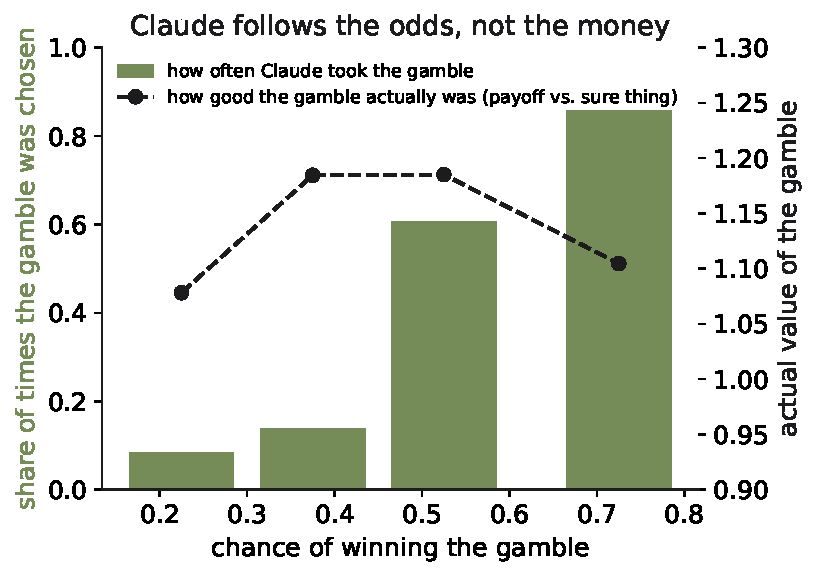
\includegraphics[width=0.8\linewidth]{fig3_empirical_p1.pdf}
\caption*{\small\textbf{Figure 1. The Phase 1 diagnostic: chasing the odds, not the prize.} Bets are
grouped by their chance of winning, from low on the left to high on the right. The bars show how often
the model took the gamble in each group: gamble-taking climbs from about 8 percent to about 86 percent
as the win probability rises. The dashed line is the average expected value of the gambles in each group,
and it stays roughly flat across the whole range. So the model took the gamble far more often as the odds
improved, even though the gambles were worth about the same money throughout. It is deciding on the odds
and nearly ignoring the size of the prize.}
\end{figure}

Read the figure slowly. The bars climb sharply from left to right: a higher chance of winning brings much
more gambling. The dashed line, the actual dollar value of the bets, barely moves. If the model cared
about the money, and the money stayed flat, its gambling rate should have stayed roughly flat too.
Instead it tracked the probability number almost perfectly. A pure risk-aversion model cannot do this,
which is why I added probability weighting to get model M2.

Here are M2's fitted dials.

\begin{table}[h]
\centering
\small
\caption*{\small\textbf{Phase 1, model M2.} CRRA value, Prelec weighting, position term. Estimates with
standard errors in parentheses. $n \approx 1{,}200$.}
\begin{tabular}{@{}l l >{\RaggedRight}p{2.75in}@{}}
\toprule
\textbf{Parameter} & \textbf{Estimate (give-or-take)} & \textbf{Plain reading of this row} \\
\midrule
$r$ (curvature)       & 0.592 (0.028) & Ordinary, human-like caution once the odds-distortion is removed \\
$\gamma$ (Prelec)     & 2.693 (0.166) & An extreme S-shape; the model crushes long shots toward zero \\
$\mu$ (Fechner noise) & 0.104 (0.008) & Low sloppiness; the model chooses fairly decisively \\
$\delta$ (position)   & 1.257 (0.160) & A mild leftover pull toward the option listed second \\
\bottomrule
\end{tabular}
\end{table}

The parentheses report the give-or-take on each number, which deserves its own definition.

\begin{defbox}[Standard error and confidence interval]
A \term{standard error} is the give-or-take on an estimate: how much the number would wobble if I reran
the whole experiment. A small standard error means a precise estimate. Reading the table, $r = 0.592$
with a standard error of $0.028$ means my best guess for $r$ is about $0.59$ and would typically wobble
by less than three-hundredths. A \term{confidence interval} is the plausible range built from that
give-or-take, roughly the estimate plus or minus two standard errors, so for $r$ the range runs about
$0.54$ to $0.65$: the band of values consistent with the data.
\end{defbox}

How do I know M2 is genuinely better and not merely more complicated? Adding dials always improves fit a
little, so I need a test that asks whether the improvement is real.

\begin{defbox}[Likelihood-ratio test and chi-square]
A \term{likelihood-ratio test} compares two nested models by scoring how well each explains the observed
choices, then asking whether the richer model's improvement is far larger than the extra flexibility
alone would buy. The improvement is compared against a reference curve called a \term{chi-square}
distribution; the number in parentheses, as in ``$\chi^2(2)$,'' counts the extra dials being tested (here
2). A huge chi-square value with a tiny $p$-value means the added dials genuinely help rather than
flattering the fit by luck.
\end{defbox}

For M1 against M2 the test gives $\chi^2(2) \approx 617$ with $p \approx 10^{-134}$, an improvement so
large that the added weighting and position dials are overwhelmingly warranted. The headline number is
the weighting dial: $\gamma = 2.69$ is an extreme S-shape, pointed the opposite way from the human value
of about $0.65$. The model \emph{underweights} long shots rather than overweighting them. Once that
distortion is accounted for, the underlying caution $r = 0.59$ is ordinary and sits squarely in the human
range.

\begin{figure}[h]
\centering
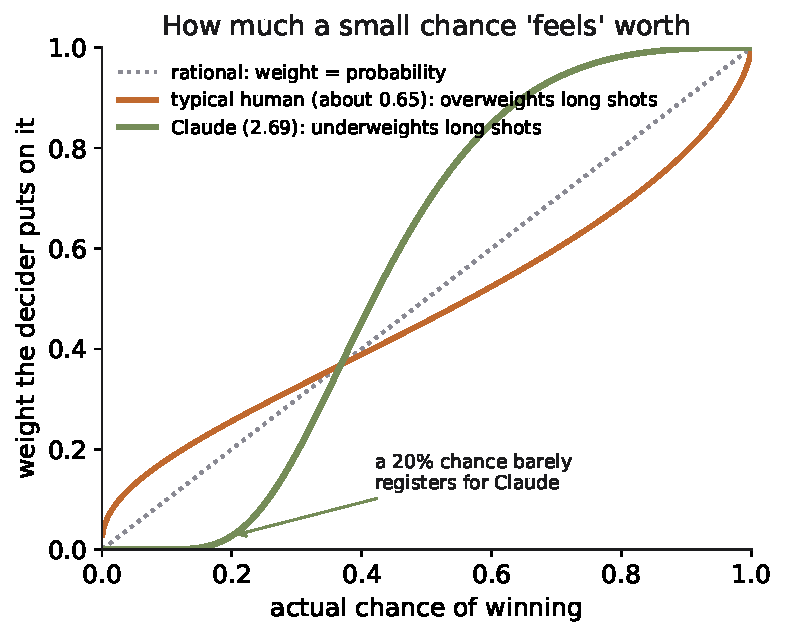
\includegraphics[width=0.8\linewidth]{fig2_weighting.pdf}
\caption*{\small\textbf{Figure 2. How the model distorts probabilities, versus a human and a perfect
decider.} The horizontal axis is the stated probability; the vertical axis is the felt probability the
decider acts on. The diagonal is a perfectly rational decider ($\gamma = 1$, felt equals stated). The
human curve ($\gamma \approx 0.65$) sits above the diagonal at the low end: people overweight small
chances, which is why lottery tickets sell. The model's curve (Claude at $\gamma = 2.69$) does the
opposite, diving below the diagonal at the low end, so it underweights small chances and treats a long
shot as even more hopeless than it is. In practical terms this model will refuse a low-chance gamble at
almost any prize.}
\end{figure}

\begin{workbox}[What $\gamma = 2.69$ does to a real chance]
Take the win probability from the example bet, $p = 0.66$, and put it through the Prelec formula with
$\gamma = 2.69$. First $-\ln(0.66) \approx 0.416$; raise it to the power $2.69$ to get about $0.098$;
then $w(0.66) = e^{-0.098} \approx 0.907$. A real 66 percent chance feels like about 91 percent to this
model. Now a long shot, $p = 0.10$: here $-\ln(0.10) \approx 2.303$, and $2.303^{2.69} \approx 9.7$, so
$w(0.10) = e^{-9.7} \approx 0.00006$. A real 1-in-10 chance feels like about 6-in-100,000, essentially
zero. That is why the model refuses long shots at any prize: the chance barely registers as real.
\end{workbox}

\begin{asidebox}[A candid note on fit]
I do not want to oversell M2. A stripped-down model that predicts the choice from the win probability
alone, ignoring dollars entirely (call it M3), nearly ties M2 on a standard model-comparison score. That
score is the \term{AIC} (Akaike Information Criterion), which rewards fit but charges a penalty for each
extra dial, so models of different sizes can be compared on a level field, with a lower score better. M3
nearly tying M2 means a simple rule-of-thumb model predicts about as well as the elaborate one. So in
Phase 1 the structural model earns its keep by being interpretable and human-comparable, mapping onto the
same primitives we measure in people, rather than by predicting better. I keep it for that reason, and I
would not claim it beats the reduced-form fit on the data alone. This is exactly what motivates the
held-out test I raise in Section 6.
\end{asidebox}

\subsection{Phase 2 results}

\textbf{The plainest result first.} Gamble-taking is 0.398 in the gain wording, 0.300 in neutral wording,
and 0.096 in the loss (mixed) wording. The loss-minus-gain difference is $-0.302$ (with $p \approx 3
\times 10^{-47}$, meaning it is not remotely a fluke). Holding each of the 40 individual bets fixed, 88
percent of them show the same drop, so it is not an artifact of which bets happened to appear where. And
the control, one sure amount plainly larger than another, is answered correctly 100 percent of the time,
which confirms the model reads dollar magnitudes perfectly well when no probability is in the way.

\begin{figure}[h]
\centering
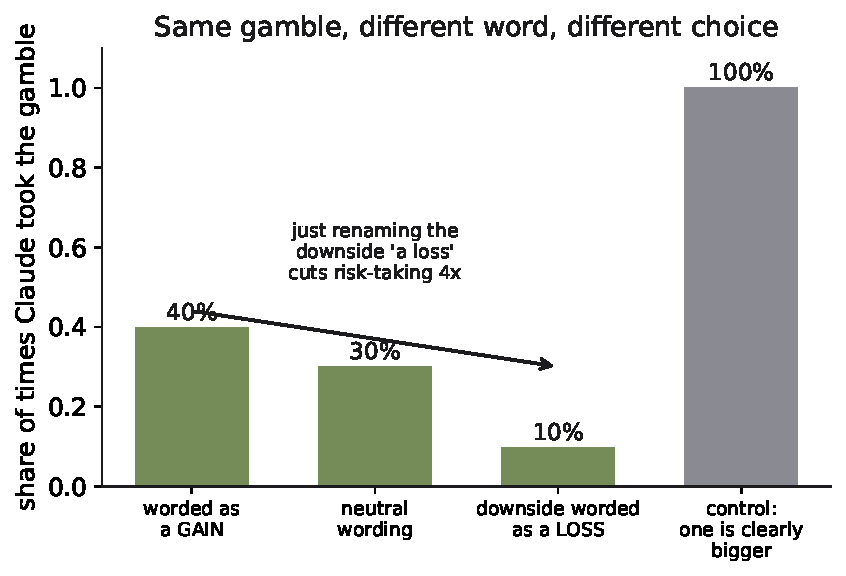
\includegraphics[width=0.8\linewidth]{fig5_framing.pdf}
\caption*{\small\textbf{Figure 3. Phase 2 framing result: one gamble, four wordings.} Each bar is how
often the model took the gamble (Option B) under a given wording. Gambling is about 40 percent in the
gain wording, about 30 percent in neutral wording, and about 10 percent when the downside is called a
loss. The rightmost bar is the control, answered correctly 100 percent of the time. The gain and loss
wordings imply identical final wealth, yet gamble-taking falls from 40 percent to 10 percent on the mere
presence of the word ``loss.'' Because the control is at ceiling, this is not an arithmetic failure; the
pull is specific to loss-worded risk.}
\end{figure}

The control does real work here. Because the model nailed it 100 percent of the time, I know the framing
effect is not the model being bad at arithmetic. The pull comes specifically from the loss wording. To
put a number on the fear of losses behind it, I fit the reference-dependent model under the standard
assumption that the stated wording sets the reference point ($\phi = 1$).

\begin{table}[h]
\centering
\small
\caption*{\small\textbf{Phase 2, structural estimate (stated-reference version).} Estimates with standard
errors in parentheses. $n \approx 2{,}480$.}
\begin{tabular}{@{}l l >{\RaggedRight}p{2.75in}@{}}
\toprule
\textbf{Parameter} & \textbf{Estimate (give-or-take)} & \textbf{Plain reading of this row} \\
\midrule
$\lambda$ (fear of losses) & 3.234 (0.171) & A loss looms about $3.2\times$ larger than an equal gain \\
$\alpha$ (curvature)       & 0.503 (0.024) & Value flattens as amounts grow; a human-plausible bend \\
$\gamma$ (Prelec)          & 1.516 (0.059) & A mild S-shape; long shots still somewhat underweighted \\
\bottomrule
\end{tabular}
\end{table}

The formal test of $\lambda = 1$ (no loss aversion) is decisively rejected, with a $z$ of about 13. For
comparison, a typical human sits near $\lambda \approx 2.25$, near $\gamma \approx 0.65$ on weighting, and
near $\alpha \approx 0.88$ on curvature. The model's $\lambda = 3.23$ puts it \emph{above} the usual human
level of loss aversion.

\begin{figure}[h]
\centering
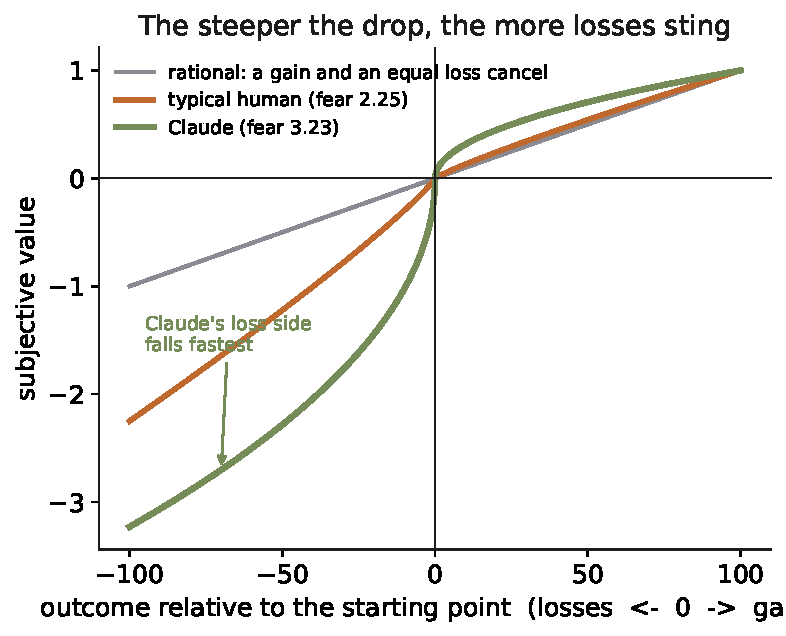
\includegraphics[width=0.8\linewidth]{fig4_lossaversion.pdf}
\caption*{\small\textbf{Figure 4. The value function, model versus human versus rational.} The horizontal
axis is the outcome measured from the reference point, losses to the left and gains to the right; the
vertical axis is felt value. The rational (symmetric) line treats a loss and an equal gain as mirror
images. The human curve ($\lambda = 2.25$) drops more steeply on the loss side than it rises on the gain
side. The model's curve (Claude at $\lambda = 3.23$) drops the most steeply of the three: it fears losses
even more than a typical person does, which is why relabeling the downside as a loss drove its gambling
from about 40 percent to about 10 percent.}
\end{figure}

\subsection{The validation-arm result}

Recall the validation check: on a slice of trials I let the model answer in free text instead of the
forced A-or-B form. The two modes do not agree uniformly, and the disagreement is itself informative.

\begin{asidebox}[The forced form and free text do not always agree]
\textbf{Phase 1 agrees.} Free-text gamble-taking is 0.61 against 0.55 under the forced form (from 130
free-text trials), a difference small enough to be noise ($p = 0.19$). For Phase 1, forcing the form was
a clean measuring device.

\smallskip
\textbf{Phase 2 diverges sharply.} Split the framing gap (gain minus loss) by how the model answered.
Under the forced form the gap is $+0.33$ (gambling 0.385 in the gain wording, 0.057 in the loss wording).
Under free text it shrinks to only $+0.09$ (0.527 gain, 0.434 loss). Letting the model reply in free text,
which gives it room to reason a little before committing, sharply shrinks the framing effect. So the large
framing result I found in Phase 2 depends heavily on the forced, immediate-answer format. This fits a
known pattern in humans, that giving a decider room to deliberate reduces how much wording sways them, and
it is both a caveat on the Phase 2 magnitude and arguably a finding in its own right.

\smallskip
\textbf{Two honest caveats.} The free-text slice is smaller (about 74 to 83 usable choices per wording),
and its usable subset may be skewed, because I keep only replies that open with a bare letter and discard
any that begin with reasoning like ``I would choose.'' That motivates a dedicated reason-then-answer
follow-up. The framing gap under the forced form remains a valid result for the immediate-choice setting.
What depends on the format is the \emph{size} of the effect, not its existence.
\end{asidebox}

The lesson is plain: how large the framing effect looks depends on how you ask. Force a snap answer and
the wording moves the model a lot; allow a moment of reasoning and the wording moves it much less.

\subsection{A limit on what the data can tell apart}

The Phase 2 numbers come with an honest limit, and I want to be upfront about it.

\begin{asidebox}[Two stories the data cannot separate]
The loss-wording effect has two explanations that predict almost the same choices. One story: the model
\emph{moved its reference point}. Told ``you have been given \$162,'' it now treats \$162 as the new
baseline, so the downside reads as a loss (this is the $\phi$ dial being high). The other story: the model
simply \emph{has an extreme fear of losses} (a high $\lambda$), with the baseline barely moving. Because
both stories bend the same choices the same way, the data cannot cleanly vote between them. Formally, the
$\lambda$ dial and the $\phi$ dial are tangled together, a problem called \term{collinearity}: the
estimator can trade one off against the other without changing the fit. The analogy: if I tell you two
numbers multiply to 12, you cannot tell whether they are 3 and 4 or 2 and 6. Knowing the product does not
pin down the pair. When I let $\phi$ float, the fitting procedure duly slides to a corner ($\phi$ toward 0
with $\lambda$ pinned at its limit), a telltale sign the two are not separately identified.

\smallskip
So the trustworthy headline is the plain, assumption-free fact: gambling fell from 40 percent to 10
percent when the downside was worded as a loss. That gap holds no matter which story is true. I report the
$\lambda = 3.23$ figure under the standard assumption ($\phi = 1$), state the tangle openly, and do not
report a free-$\phi$ number, because I do not believe it is identified. Treat the 40-to-10 gap as the
rock, and the 3.23 as a reasonable reading resting on one modeling choice.
\end{asidebox}

A related caution concerns the position dial $\delta$, which I always include but never interpret. Such a
control has a name.

\begin{defbox}[Nuisance parameter]
A \term{nuisance parameter} is a dial I put in the model to soak up some unwanted effect, but that I do
not interpret as a real preference. The position dial $\delta$ is one: it exists so that a mild habit of
favoring a listed position does not contaminate the dials I care about.
\end{defbox}

I treat $\delta$ as a nuisance for a concrete reason: it flips sign between the two phases, from $+1.26$ in
Phase 1 to $-0.36$ in Phase 2. A genuine, stable trait of the model would not flip like that. The flip
tells me position bias is an artifact of the specific layouts, so I carry $\delta$ as a control rather than
read anything into it.

% ============================================================
%  5. THREATS TO VALIDITY
% ============================================================
\section{What could go wrong: threats to validity}

Any careful experiment should list the ways it might mislead. Here is my checklist, in plain terms.

\begin{enumerate}[leftmargin=1.5em]
\item \textbf{No real stakes.} The choices are hypothetical: nothing is actually paid out. So I do not
claim to measure incentivized preferences. I read every number as a property of how the model responds
under this exact protocol, not as proof of an inner desire. This is the limit I would most like to fix,
and I return to it in Section 6.
\item \textbf{Contamination.} Handled by the odd, off-textbook numbers of Section 3.1. By construction the
bets are not ones the model could have memorized.
\item \textbf{Wording sensitivity.} Handled by the five paraphrases, which let me measure how much wording
matters rather than pretend it does not.
\item \textbf{Is temperature the right kind of noise?} Flagged in Section 3.3. I treat the model's
run-to-run randomness as the choice noise $\mu$, and I concede that whether this is truly the right sort
of noise for an economic model is unsettled. Phase 3 removes the reliance on it by reading choices off the
log-probabilities.
\item \textbf{The model changing underneath me.} Handled by pinning the dated snapshot
\texttt{claude-\allowbreak haiku-\allowbreak 4-\allowbreak 5-\allowbreak 20251001}, so the subject does not silently update mid-experiment.
\item \textbf{Not over-reading the model's ``mind.''} I do not claim the model has feelings or beliefs. I
frame every estimate as a property of its response pattern under this protocol, nothing more.
\end{enumerate}

% ============================================================
%  6. OPEN QUESTIONS
% ============================================================
\section{Open questions I am still working through}

These are the four questions I am genuinely wrestling with. I state each plainly.

\begin{enumerate}[leftmargin=1.5em]
\item \textbf{Can a model's choices ever be given real stakes?} In human experiments we make choices
matter with real money. A language model has no wealth and nothing to spend, so those mechanisms do not
transfer, and the current consensus treats a model's choices as hypothetical. I can see two speculative
routes to giving a choice genuine consequence for the model. One is to embed the bet inside a larger task
so the payoff is something the model actually tries to optimize, such as its remaining task budget or its
score. The other is to train the model beforehand so that resources genuinely matter to it. I am not sure
either is truly defensible, and I would like a considered view on whether the honest ceiling here is simply
``hypothetical, unincentivized choices.''
\item \textbf{Can I untangle the fear of losses from the moving reference point?} The clean fix for the
$\lambda$-versus-$\phi$ tangle would be a design where the two leave different fingerprints, for example
bets that straddle the reference point at several different anchor amounts, so the two dials cannot mimic
each other. I sketch that design but am not certain it fully works, and I would welcome a better instrument.
\item \textbf{Is temperature-as-noise defensible at all?} Should I keep treating the model's token-level
randomness as choice noise, or abandon that reading entirely in favor of the Phase 3 log-probability
readout, and treat the Phase 1 and Phase 2 sampled-choice estimates as provisional?
\item \textbf{Should I add a held-out prediction test?} By this I mean fitting the Phase 1 weighting model
on part of the bets (say 30 of the 40) and then predicting the model's choices on the 10 bets it never saw
during fitting. Because the stripped-down M3 nearly ties the structural M2 on AIC, an overfitting worry is
natural, and this test would show directly whether the estimated probability-weighting is real structure or
fitted noise. Is it worth adding?
\end{enumerate}

\vspace{6pt}
{\color{rulegray}\rule{\linewidth}{0.8pt}}\\[3pt]
{\footnotesize\color{mutegray} Every estimate here is a property of one pinned model snapshot under this
particular hypothetical, forced-choice protocol, in which the model chose among amounts with nothing
actually at stake. They are a careful measurement of that setting, not a claim about every AI system
everywhere. Thank you for reading.}

\end{document}
